% SPDX-License-Identifier: CC-BY-SA-4.0
%
% Copyright (c) 2020 Philipp Le
%
% Except where otherwise noted, this work is licensed under a
% Creative Commons Attribution-ShareAlike 4.0 License.
%
% Please find the full copy of the licence at:
% https://creativecommons.org/licenses/by-sa/4.0/legalcode

\phantomsection
\addcontentsline{toc}{section}{Exercise 2}
\section*{Exercise 2}

\begin{question}[subtitle={Mono-chromatic Signals}]
	A mono-chromatic signal $u(t)$ is given:
	\begin{equation*}
		u(t) = \SI{2}{V} \cdot \cos\left(2 \pi \cdot \SI{1}{MHz} \cdot t + \frac{\pi}{2} \right)
	\end{equation*}
	\begin{tasks}
		\task
		How much is the frequency and angular frequency? How much is the amplitude? How much is the phase?
		\task
		Give the phasor of the signal!
		\task
		An DC bias is added to the signal $u(t)$.
		\begin{equation*}
			u_2(t) = \SI{1}{V} + \SI{2}{V} \cdot \cos\left(2 \pi \cdot \SI{1}{MHz} \cdot t + \frac{\pi}{2} \right)
		\end{equation*}
		Is the resulting signal $u_2(t)$ still mono-chromatic?
	\end{tasks}
\end{question}

\begin{solution}
	\begin{tasks}
		\task
		\begin{itemize}
			\item Frequency: \SI{1}{MHz}
			\item Angular frequency: $2 \pi \cdot \SI{1}{MHz} = \SI{6283185.3}{s^{-1}}$
			\item Phase: $\pi/2 \si{rad}$ or \SI{-90}{\degree}
			\item Amplitude: \SI{2}{V}
		\end{itemize}
		\task
		$\underline{U} = \SI{2}{V} \cdot e^{+j \frac{\pi}{2}}$ or $\underline{U} = \SI{2}{V} \angle +\frac{\pi}{2}$
		\task
		No, the DC bias adds a mono-chromatic component with a frequency of $f = 0$. $u_2(t)$ is a Fourier series.
	\end{tasks}
\end{solution}

\begin{question}[subtitle={Fourier Series}]
	The following periodic signal is given.
	\begin{figure}[H]
		\centering
		\begin{tikzpicture}
			\begin{axis}[
				height={0.25\textheight},
				width=0.8\linewidth,
				scale only axis,
				xlabel={$t \text{ in } \si{s}$},
				ylabel={$x(t) \text{ in } \si{V}$},
				%grid style={line width=.6pt, color=lightgray},
				%grid=both,
				grid=none,
				legend pos=north east,
				axis y line=middle,
				axis x line=middle,
				every axis x label/.style={
					at={(ticklabel* cs:1.05)},
					anchor=north,
				},
				every axis y label/.style={
					at={(ticklabel* cs:1.05)},
					anchor=east,
				},
				xmin=-3.5,
				xmax=3.5,
				ymin=-0.5,
				ymax=1.1,
				xtick={-3.0, -2.5, ..., 3.0},
				%ytick={0, 0.5, ..., 1.5},
				%xticklabels={0, 1, $t_0$, 3, 4, ..., 10}
			]
				\addplot[blue, thick] coordinates {(-3.0,-0.2) (-2.5,-0.2)};
				\addplot[blue, thick] coordinates {(-2.5,0.8) (-1.5,0.8)};
				\addplot[blue, thick] coordinates {(-1.5,-0.2) (-0.5,-0.2)};
				\addplot[blue, thick] coordinates {(-0.5,0.8) (0.5,0.8)};
				\addplot[blue, thick] coordinates {(0.5,-0.2) (1.5,-0.2)};
				\addplot[blue, thick] coordinates {(1.5,0.8) (2.5,0.8)};
				\addplot[blue, thick] coordinates {(2.5,-0.2) (3.0,-0.2)};
				
				\addplot[blue, thick, dashed] coordinates {(-2.5,-0.2) (-2.5,0.8)};
				\addplot[blue, thick, dashed] coordinates {(-1.5,0.8) (-1.5,-0.2)};
				\addplot[blue, thick, dashed] coordinates {(-0.5,-0.2) (-0.5,0.8)};
				\addplot[blue, thick, dashed] coordinates {(0.5,0.8) (0.5,-0.2)};
				\addplot[blue, thick, dashed] coordinates {(1.5,-0.2) (1.5,0.8)};
				\addplot[blue, thick, dashed] coordinates {(2.5,0.8) (2.5,-0.2)};
			\end{axis}
		\end{tikzpicture}
	\end{figure}
	
	\begin{tasks}
		\task
		Find a functional expression for the above signal!
		\task
		What is the base frequency?
		\task
		Find the real-valued Fourier series coefficients $a_n$ and $b_m$!
		\task
		Find the complex-valued Fourier series coefficients $\underline{c}_n$!
		\task
		Plot the amplitude and phase spectra for $-5 \leq n \leq 5$!
	\end{tasks}
\end{question}

\begin{solution}
	\begin{tasks}
		\task
		\begin{equation*}
			x(t) = \begin{cases}
				\SI{0.8}{V}, &\quad \text{ if} \; \left(-\frac{T_0}{4} + n \cdot T_0\right) \leq t < \left(\frac{T_0}{4} + n \cdot T_0\right) \\
				\SI{-0.2}{V}, &\quad \text{ if} \; \left(\frac{T_0}{4} + n \cdot T_0\right) \leq t < \left(\frac{3T_0}{4} + n \cdot T_0\right) \\
			\end{cases} \qquad \forall \; n \in \mathbb{Z}
		\end{equation*}
		
		with $T_0 = \SI{2}{s}$
		
		\task
		\begin{itemize}
			\item Period: $T_0 = \SI{2}{s}$
			\item Base frequency: $f_0 = \SI{0,5}{Hz}$
			\item Base angular frequency: $\omega_0 = \SI{3.14}{s^{-1}}$
		\end{itemize}
	
		\task
		\begin{equation*}
			\begin{split}
				a_n &= \frac{2}{T_0} \left( \int\limits_{-\frac{T_0}{4}}^{\frac{T_0}{4}} \SI{0.8}{V} \cdot \cos\left(n\frac{2\pi}{T_0}t\right) \, \mathrm{d} t - \int\limits_{\frac{T_0}{4}}^{\frac{3T_0}{4}} \SI{0.2}{V} \cdot \cos\left(n\frac{2\pi}{T_0}t\right) \, \mathrm{d} t \right) \\
				 &= \frac{2}{T_0} \frac{T_0}{2 \pi n} \left( \SI{0.8}{V} \cdot \left[\sin\left(n\frac{2\pi}{T_0}t\right)\right]_{-\frac{T_0}{4}}^{\frac{T_0}{4}} - \SI{0.2}{V} \cdot \left[\sin\left(n\frac{2\pi}{T_0}t\right)\right]_{\frac{T_0}{4}}^{\frac{3T_0}{4}} \right) \\
				 &= \frac{1}{\pi n} \left(
				 	\SI{0.8}{V} \cdot \left(
				 		\sin\left(\frac{\pi}{2}n\right)
				 		- \underbrace{\sin\left(-\frac{\pi}{2}n\right)}_{= -\sin\left(\frac{\pi}{2}n\right)}
				 	\right)
				 	- \SI{0.2}{V} \cdot \left(
				 		\underbrace{\sin\left(\frac{3\pi}{2}n\right)}_{= -\sin\left(\frac{\pi}{2}n\right)}
				 		- \sin\left(\frac{\pi}{2}n\right)
				 	\right)
				 \right) \\
				 &= \frac{2}{\pi n} \left( \SI{0.8}{V} \cdot \sin\left(\frac{\pi}{2}n\right) - \SI{0.2}{V} \cdot \sin\left(\frac{\pi}{2}n\right) \right) \\
				 &= \frac{\SI{2,0}{V}}{\pi n} \cdot \sin\left(\frac{\pi}{2}n\right) \\
				 &= \begin{cases}
				 	\frac{\SI{2,0}{V}}{\pi n} (-1)^{\frac{n+3}{2}} &\quad \; \forall n \text{ odd}, \\
				 	0 &\quad \; \forall n \text{ even}.
				 \end{cases}
			\end{split}
		\end{equation*}
		
		$a_0$ (DC bias) needs special treatment.
		\begin{equation*}
			\begin{split}
				a_0 &= \frac{1}{T_0} \left( \int\limits_{-\frac{T_0}{4}}^{\frac{T_0}{4}} \SI{0.8}{V} \, \mathrm{d} t - \int\limits_{\frac{T_0}{4}}^{\frac{3T_0}{4}} \SI{0.2}{V}  \, \mathrm{d} t \right) \\
				 &= \frac{1}{T_0} \left( \SI{0.8}{V} \cdot \left[t\right]_{-\frac{T_0}{4}}^{\frac{T_0}{4}} - \SI{0.2}{V} \cdot \left[t\right]_{\frac{T_0}{4}}^{\frac{3T_0}{4}} \right) \\
				 &= \frac{1}{T_0} \left( \SI{0.8}{V} \cdot \left(\frac{T_0}{4} - \left(-\frac{T_0}{4}\right)\right) - \SI{0.2}{V} \cdot \left(\frac{3T_0}{4} - \frac{T_0}{4}\right) \right) \\
				 &= \frac{1}{T_0} \left( \SI{0.8}{V} \cdot \frac{T_0}{2} - \SI{0.2}{V} \cdot \frac{T_0}{2} \right) \\
				 &= \SI{0.3}{V}
			\end{split}
		\end{equation*}
		
		\begin{equation*}
			\begin{split}
				b_n &= \frac{2}{T_0} \left( \int\limits_{-\frac{T_0}{4}}^{\frac{T_0}{4}} \SI{0.8}{V} \cdot \sin\left(n\frac{2\pi}{T_0}t\right) \, \mathrm{d} t - \int\limits_{\frac{T_0}{4}}^{\frac{3T_0}{4}} \SI{0.2}{V} \cdot \sin\left(n\frac{2\pi}{T_0}t\right) \, \mathrm{d} t \right) \\
				 &= \frac{2}{T_0} \frac{T_0}{2 \pi n} \left( \SI{0.8}{V} \cdot \left[-\cos\left(n\frac{2\pi}{T_0}t\right)\right]_{-\frac{T_0}{4}}^{\frac{T_0}{4}} - \SI{0.2}{V} \cdot \left[-\cos\left(n\frac{2\pi}{T_0}t\right)\right]_{\frac{T_0}{4}}^{\frac{3T_0}{4}} \right) \\
				 &= \frac{1}{\pi n} \left(
					\SI{0.8}{V} \cdot \left(
						-\cos\left(\frac{\pi}{2}n\right)
						+ \underbrace{\cos\left(-\frac{\pi}{2}n\right)}_{= \cos\left(\frac{\pi}{2}n\right)}
					\right)
					- \SI{0.2}{V} \cdot \left(
						-\underbrace{\cos\left(\frac{3\pi}{2}n\right)}_{= \cos\left(\frac{\pi}{2}n\right)}
						+ \cos\left(\frac{\pi}{2}n\right)
					\right)
				\right) \\
				 &= 0
			\end{split}
		\end{equation*}
		
		\task
		$\underline{c}_n$:
		\begin{equation*}
			\begin{split}
				b_n &= \frac{1}{T_0} \left( \int\limits_{-\frac{T_0}{4}}^{\frac{T_0}{4}} \SI{0.8}{V} \cdot e^{-j n\frac{2\pi}{T_0}t} \, \mathrm{d} t - \int\limits_{\frac{T_0}{4}}^{\frac{3T_0}{4}} \SI{0.2}{V} \cdot e^{-j n\frac{2\pi}{T_0}t} \, \mathrm{d} t \right) \\
				&= \frac{1}{T_0} \frac{T_0}{2 \pi n (-j)} \left(
					\SI{0.8}{V} \cdot \left[e^{-j n\frac{2\pi}{T_0}t}\right]_{-\frac{T_0}{4}}^{\frac{T_0}{4}}
					- \SI{0.2}{V} \cdot \left[e^{-j n\frac{2\pi}{T_0}t}\right]_{\frac{T_0}{4}}^{\frac{3T_0}{4}}
				\right) \\
				&= j \frac{1}{2 \pi n} \left(
					\SI{0.8}{V} \left(
						e^{-j n\frac{\pi}{2}}
						- e^{+j n\frac{\pi}{2}}
					\right)
					- \SI{0.2}{V} \left(
						e^{-j n\frac{3 \pi}{2}}
						- e^{-j n\frac{\pi}{2}}
					\right)
				\right) \\
				&=  \begin{cases}
					\frac{\SI{1,0}{V}}{\pi n} e^{j\frac{n+3}{2}\pi} &\quad \; \forall n \text{ odd}, \\
					0 &\quad \; \forall n \text{ even}.
				\end{cases}
			\end{split}
		\end{equation*}
		Following has been used:
		\begin{equation*}
			\begin{split}
				\left(e^{-j n\frac{\pi}{2}} - e^{+j n\frac{\pi}{2}}\right) &= \begin{cases}
					-j &\quad \forall n = 4 k + 1, k \in \mathbb{Z}, \\
					+j &\quad \forall n = 4 k + 3, k \in \mathbb{Z}, \\
					0 &\quad \forall n = 2 k, k \in \mathbb{Z}.
				\end{cases} \\
				\left(e^{-j n\frac{3 \pi}{2}} - e^{-j n\frac{\pi}{2}}\right) &= \begin{cases}
					+j &\quad \forall n = 4 k + 1, k \in \mathbb{Z}, \\
					-j &\quad \forall n = 4 k + 3, k \in \mathbb{Z}, \\
					0 &\quad \forall n = 2 k, k \in \mathbb{Z}.
				\end{cases}
			\end{split}
		\end{equation*}
		
		\task
		\begin{figure}[H]
			\centering
			\begin{tikzpicture}
				\begin{axis}[
					height={0.25\textheight},
					width=0.9\linewidth,
					scale only axis,
					xlabel={$n$},
					ylabel={$\left|\underline{c}_n\right| in \si{V}$},
					%grid style={line width=.6pt, color=lightgray},
					%grid=both,
					grid=none,
					legend pos=north east,
					axis y line=middle,
					axis x line=middle,
					every axis x label/.style={
						at={(ticklabel* cs:1.05)},
						anchor=north,
					},
					every axis y label/.style={
						at={(ticklabel* cs:1.05)},
						anchor=east,
					},
					xmin=-5.5,
					xmax=5.5,
					xtick={-5, -4, ..., 5},
					ymin=0,
					ymax=0.45,
					ytick={0, 0.1, ..., 0.4}
				]
					\addplot[red, thick] coordinates {(-5,0) (-5,0.064)};
					\addplot[red, thick] coordinates {(-3,0) (-3,0.106)};
					\addplot[red, thick] coordinates {(-1,0) (-1,0.318)};
					\addplot[red, thick] coordinates {(0,0) (0,0.3)};
					\addplot[red, thick] coordinates {(1,0) (1,0.318)};
					\addplot[red, thick] coordinates {(3,0) (3,0.106)};
					\addplot[red, thick] coordinates {(5,0) (5,0.064)};
					
					\addplot[red, thick, only marks, mark=o] coordinates {(-5,0.064)};
					\addplot[red, thick, only marks, mark=o] coordinates {(-4,0)};
					\addplot[red, thick, only marks, mark=o] coordinates {(-3,0.106)};
					\addplot[red, thick, only marks, mark=o] coordinates {(-2,0)};
					\addplot[red, thick, only marks, mark=o] coordinates {(-1,0.318)};
					\addplot[red, thick, only marks, mark=o] coordinates {(0,0.3)};
					\addplot[red, thick, only marks, mark=o] coordinates {(1,0.318)};
					\addplot[red, thick, only marks, mark=o] coordinates {(2,0)};
					\addplot[red, thick, only marks, mark=o] coordinates {(3,0.106)};
					\addplot[red, thick, only marks, mark=o] coordinates {(4,0)};
					\addplot[red, thick, only marks, mark=o] coordinates {(5,0.064)};
				\end{axis}
			\end{tikzpicture}
		\end{figure}
	
		\begin{figure}[H]
			\centering
			\begin{tikzpicture}
				\begin{axis}[
					height={0.25\textheight},
					width=0.9\linewidth,
					scale only axis,
					xlabel={$\omega \text{ in } \si{s^{-1}}$},
					ylabel={$\left|\underline{H}\left(j \omega\right)\right|$},
					%grid style={line width=.6pt, color=lightgray},
					%grid=both,
					grid=none,
					legend pos=north east,
					axis y line=middle,
					axis x line=middle,
					every axis x label/.style={
						at={(ticklabel* cs:1.05)},
						anchor=north,
					},
					every axis y label/.style={
						at={(ticklabel* cs:1.05)},
						anchor=east,
					},
					xmin=-5.5,
					xmax=5.5,
					ymin=-3.5,
					ymax=3.5,
					ytick={-3.14159, -1.5708, 1.5708, 3.14159},
					yticklabels={$-\pi\hspace{0.30cm}$, $-\frac{\pi}{2}$, $\frac{\pi}{2}$, $\pi\hspace{0.10cm}$},
				]
					\addplot[red, thick] coordinates {(-5,0) (-5,0)};
					\addplot[red, thick] coordinates {(-3,0) (-3,-3.14159)};
					\addplot[red, thick] coordinates {(-1,0) (-1,0)};
					\addplot[red, thick] coordinates {(0,0) (0,0)};
					\addplot[red, thick] coordinates {(1,0) (1,0)};
					\addplot[red, thick] coordinates {(3,0) (3,3.14159)};
					\addplot[red, thick] coordinates {(5,0) (5,0)};
					
					\addplot[red, thick, only marks, mark=o] coordinates {(-5,0)};
					\addplot[red, thick, only marks, mark=o] coordinates {(-4,0)};
					\addplot[red, thick, only marks, mark=o] coordinates {(-3,-3.14159)};
					\addplot[red, thick, only marks, mark=o] coordinates {(-2,0)};
					\addplot[red, thick, only marks, mark=o] coordinates {(-1,0)};
					\addplot[red, thick, only marks, mark=o] coordinates {(0,0)};
					\addplot[red, thick, only marks, mark=o] coordinates {(1,0)};
					\addplot[red, thick, only marks, mark=o] coordinates {(2,0)};
					\addplot[red, thick, only marks, mark=o] coordinates {(3,3.14159)};
					\addplot[red, thick, only marks, mark=o] coordinates {(4,0)};
					\addplot[red, thick, only marks, mark=o] coordinates {(5,0)};
				\end{axis}
			\end{tikzpicture}
		\end{figure}
	
		%TODO
	\end{tasks}
\end{solution}

\begin{question}[subtitle={Using the Fourier Transform}]
	Derive the Fourier transform, without using the duality, of
	\begin{tasks}
		\task
		the time shift
		\begin{equation*}
			\mathcal{F}\left\{\underline{f}(t - t_0)\right\}
		\end{equation*}
		
		\task
		the frequency shift
		\begin{equation*}
			\mathcal{F}\left\{e^{j \omega_0 t} \underline{f}(t)\right\}
		\end{equation*}
		
		%\task
		%Derive the Fourier transform of the frequency shift using the time shift and duality!
	\end{tasks}
\end{question}

\begin{solution}
	\begin{tasks}
		\task
		Let
		\begin{equation*}
			\underline{h}(t) = \underline{f}(t - t_0)
		\end{equation*}
		The Fourier transform:
		\begin{equation*}
			\mathcal{F}\left\{\underline{h}(t)\right\} = \int\limits_{t = -\infty}^{\infty} \underline{f}(t - t_0) \cdot e^{-j \omega t} \, \mathrm{d} t
		\end{equation*}
		Substitute $t' = (t - t_0)$ in the integral.
		\begin{equation*}
			\mathcal{F}\left\{\underline{h}(t)\right\} = \int\limits_{t' = -\infty}^{\infty} \underline{f}(t') \cdot e^{-j \omega (t' + t_0)} \, \mathrm{d} t'
		\end{equation*}
		$e^{-j \omega t_0}$ is a constant.
		\begin{equation*}
			\mathcal{F}\left\{\underline{h}(t)\right\} = e^{-j \omega t_0} \underbrace{\int\limits_{t' = -\infty}^{\infty} \underline{f}(t') \cdot e^{-j \omega t'} \, \mathrm{d} t'}_{= \mathcal{F}\left\{\underline{f}(t)\right\} }
		\end{equation*}
		
		\task
		Let
		\begin{equation*}
			\underline{h}(t) = e^{j \omega_0 t} \underline{f}(t)
		\end{equation*}
		The Fourier transform:
		\begin{equation*}
			\mathcal{F}\left\{\underline{h}(t)\right\} = \int\limits_{t = -\infty}^{\infty} e^{j \omega_0 t} \underline{f}(t) \cdot e^{-j \omega t} \, \mathrm{d} t
		\end{equation*}
		Factor out $j t$ in the $e$-function.
		\begin{equation*}
			\mathcal{F}\left\{\underline{h}(t)\right\} = \int\limits_{t = -\infty}^{\infty} \underline{f}(t) \cdot e^{-j (\omega - \omega_0) t} \, \mathrm{d} t
		\end{equation*}
		Substitute $\omega' = \omega - \omega_0$ in the integral.
		\begin{equation*}
			\mathcal{F}\left\{\underline{h}(t)\right\} = \underbrace{\int\limits_{t = -\infty}^{\infty} \underline{f}(t) \cdot e^{-j \omega' t} \, \mathrm{d} t}_{= \mathcal{F}\left\{\underline{f}(t)\right\}}
		\end{equation*}
		\begin{equation*}
			\mathcal{F}\left\{\underline{h}(t)\right\} = \underline{F}\left(j \omega' \right) = \underline{F}\left(j \left(\omega - \omega_0\right) \right)
		\end{equation*}
		
%		\task
%		Let
%		\begin{equation*}
%			\underline{g}(t) = \underline{f}(t - t_0)
%		\end{equation*}
%		We know from a) that
%		\begin{equation*}
%			\underline{G}\left(\omega \right) = \mathcal{F}\left\{\underline{g}(t)\right\} = e^{-j \omega t_0} \cdot \underline{F}\left(\omega \right)
%		\end{equation*}
%		Now, swap $\omega$ and $t$, swap $t_0$ and $\frac{\omega_0}{2 \pi}$, and assume both $\underline{G}$ and $\underline{F}$ are time-domain functions from now on. $\underline{F}$ now represents the original time-domain function which is shifted in frequency.
%		\begin{equation*}
%			\underline{G}\left(t\right) = e^{- j \frac{\omega_0}{2 \pi} t} \cdot \underline{F}\left(t \right)
%		\end{equation*}
%		We already know $\underline{g}$. Assume that both $\underline{g}$ and $\underline{f}$ are frequency-domain functions now. Therefore, swap $\omega$ and $t$, ans swap $t_0$ and $\frac{2 \pi}{\omega_0}$, too.
%		\begin{equation*}
%			\mathcal{F}\left\{\underline{G}(t)\right\} = 2 \pi \cdot \underline{g}\left(- \omega\right) = \underline{f}\left(- \omega + \omega_0\right) = \underline{f}\left(\omega - \omega_0\right)
%		\end{equation*}
%		
%		We obtain the same result as in b). The duality works. \acs{QED}
	\end{tasks}
\end{solution}

\begin{question}[subtitle={Fourier Transform of Signals}]
	The following signal is given!
	\begin{equation*}
		\underline{x}(t) = j \cos\left(\omega_0 t\right) - \sin\left(\omega_0 t\right)
	\end{equation*}
	
	\begin{tasks}
		\task
		What is the Fourier transform of the signal?
		\task
		Plot the amplitude and phase spectra!
		\task
		Why does the spectrum not fulfil the symmetry rules?
	\end{tasks}
\end{question}

\begin{solution}
	\begin{tasks}
		\task
		\begin{equation*}
			\underline{X}\left(j \omega\right) = j 2 \pi \delta\left(\omega - \omega_0\right)
		\end{equation*}
		
		\task
		\begin{minipage}{0.45\linewidth}
			\begin{figure}[H]
				\centering
				\begin{tikzpicture}
					\begin{axis}[
						height={0.25\textheight},
						width=0.9\linewidth,
						scale only axis,
						xlabel={$\omega \text{ in } \si{s^{-1}}$},
						ylabel={$\left|\underline{X}\left(j \omega\right)\right| \text{ in } \si{V/Hz}$},
						%grid style={line width=.6pt, color=lightgray},
						%grid=both,
						grid=none,
						legend pos=north east,
						axis y line=middle,
						axis x line=middle,
						every axis x label/.style={
							at={(ticklabel* cs:1.05)},
							anchor=north,
						},
						every axis y label/.style={
							at={(ticklabel* cs:1.05)},
							anchor=east,
						},
						xmin=-2.5,
						xmax=2.5,
						ymin=0,
						ymax=6.5,
						xtick={-1, 0, 1},
						xticklabels={$-\omega_0$, 0, $\omega_0$},
						ytick={0, 6.28},
						yticklabels={0, 6.28},
					]
						\addplot[blue, thick] coordinates {(1,0) (1,6.28)};
						\addplot[blue, thick, only marks, mark=o] coordinates {(1,6.28)};
					\end{axis}
				\end{tikzpicture}
			\end{figure}
		\end{minipage}
		\hfill
		\begin{minipage}{0.45\linewidth}
			\begin{figure}[H]
				\centering
				\begin{tikzpicture}
					\begin{axis}[
						height={0.25\textheight},
						width=0.9\linewidth,
						scale only axis,
						xlabel={$\omega \text{ in } \si{s^{-1}}$},
						ylabel={$\arg\left(\underline{X}\left(j \omega\right)\right) \text{ in } \si{\degree}$},
						%grid style={line width=.6pt, color=lightgray},
						%grid=both,
						grid=none,
						legend pos=north east,
						axis y line=middle,
						axis x line=middle,
						every axis x label/.style={
							at={(ticklabel* cs:1.05)},
							anchor=north,
						},
						every axis y label/.style={
							at={(ticklabel* cs:1.05)},
							anchor=east,
						},
						xmin=-2.5,
						xmax=2.5,
						ymin=-3.5,
						ymax=3.5,
						xtick={-1, 0, 1},
						xticklabels={$-\omega_0$, 0, $\omega_0$},
						ytick={-3.14, -1.57, 0, 1.57, 3.14},
						yticklabels={$-\pi$, $-\frac{\pi}{2}$, 0, $\frac{\pi}{2}$, $\pi$},
					]
						\addplot[blue, thick] coordinates {(1,0) (1,1.57)};
						\addplot[blue, thick, only marks, mark=o] coordinates {(1,1.57)};
					\end{axis}
				\end{tikzpicture}
			\end{figure}
		\end{minipage}
		
		\task
		The signal is complex-valued. The symmetry rules only apply for real-valued signals.
	\end{tasks}
\end{solution}

\begin{question}[subtitle={System Analysis}]
	The following circuit is given.
	\begin{figure}[H]
		\centering
		\begin{circuitikz}
			\draw (0, 0) to[L, l=$L$, o-] ++(2,0) to[short, *-o] ++(2,0);
			\draw (2, 0) to[C, l=$C$, -*] ++(0,-2);
			\draw (0, -2) to[short, o-o] ++(4,0);
			
			\draw (0, 0) to[open, v=$u_i(t)$] (0, -2);
			\draw (4, 0) to[open, v^=$u_o(t)$] (4, -2);
		\end{circuitikz}
	\end{figure}
	\begin{tasks}
		\task
		Find a differential equation which connects $u_i(t)$ and $u_o(t)$!
		\task
		Determine the transfer function $\underline{H} \left(j \omega\right)$!
		%\task
		%Calculate the impulse response!
		\task
		Is the system causal? Why?
		\task
		What filter characteristic does the circuit have? Which order does the system have?
	\end{tasks}
\end{question}

\begin{solution}
	\begin{tasks}
		\task
		Network analysis:
		\begin{figure}[H]
			\centering
			\begin{circuitikz}
				\draw (0, 0) to[L, l=$L$, v=$u_L(t)$, i=$i_C(t)$, o-] ++(2,0) to[short, i=$i_o(t)$, *-o] ++(2,0);
				\draw (2, 0) to[C, l=$C$, i=$i_C(t)$, -*] ++(0,-2);
				\draw (0, -2) to[short, o-o] ++(4,0);
				
				\draw (0, 0) to[open, v=$u_i(t)$] (0, -2);
				\draw (4, 0) to[open, v^=$u_o(t)$] (4, -2);
			\end{circuitikz}
		\end{figure}
		\begin{itemize}
			\item Kirchhoff's current law at the only point in the circuit:
			\begin{equation*}
				i_L(t) = i_C(t) + i_o(t)
			\end{equation*}
			\item No load at the output: $i_o(t) = 0$
			\item Kirchhoff's coltage law at the only closed loop in the circuit:
			\begin{equation*}
				u_i(t) = u_L(t) + u_o(t)
			\end{equation*}
			\item Differential equation for capacitors:
			\begin{equation*}
				i_C(t) = C \frac{\mathrm{d} u_o(t)}{\mathrm{d} t}
			\end{equation*}
			\item Differential equation for inductors:
			\begin{equation*}
				u_L(t) = L \frac{\mathrm{d} u_L(t)}{\mathrm{d} t} = L C \frac{\mathrm{d}^2 u_o(t)}{\mathrm{d} t^2}
			\end{equation*}
		\end{itemize}
		Finally,
		\begin{equation*}
			u_i(t) = L C \frac{\mathrm{d}^2 u_o(t)}{\mathrm{d} t^2} + u_o(t)
		\end{equation*}
		
		\task
		\begin{equation*}
			\begin{split}
				u_i(t) &= L C \frac{\mathrm{d}^2 u_o(t)}{\mathrm{d} t^2} + u_o(t) \\
				\underline{U}_i \left(j \omega\right) &= \left( \left(j \omega\right)^2 L C + 1 \right) \underline{U}_o \left(j \omega\right)
			\end{split}
		\end{equation*}
		\begin{equation*}
			\begin{split}
			\underline{H} \left(j \omega\right) &= \frac{\underline{U}_o \left(j \omega\right)}{\underline{U}_i \left(j \omega\right)} \\
			 &= \frac{1}{\left(j \omega\right)^2 L C + 1}
			\end{split}
		\end{equation*}
		
		\task
		Yes, this is a real circuit which can be implemented with electronic components. Real components do not have knowledge of the future.
		
		\task
		Second order low pass filter
	\end{tasks}
\end{solution}

\begin{question}[subtitle={Amplitude and Phase Response}]
	\begin{figure}[H]
		\centering
		\begin{circuitikz}
			\draw (0, 0) to[C, l=$C$, o-] ++(2,0) to[short, *-o] ++(2,0);
			\draw (2, 0) to[R, l=$R$, -*] ++(0,-2);
			\draw (0, -2) to[short, o-o] ++(4,0);
			
			\draw (0, 0) to[open, v=$u_i(t)$] (0, -2);
			\draw (4, 0) to[open, v^=$u_o(t)$] (4, -2);
		\end{circuitikz}
	\end{figure}
	
	The high-pass filter has the following transfer function:
	\begin{equation}
		\underline{H}\left(j \omega\right) = \frac{j \omega RC}{j \omega RC + 1}
	\end{equation}
	with
	\begin{itemize}
		\item $R = \SI{100}{\ohm}$
		\item $C = \SI{470}{nF}$
	\end{itemize}
	
	\begin{tasks}
		\task
		Which order does the system have?
		\task
		What are the poles and zeroes of the system? Is the system stable?
		\task
		Determine and plot the amplitude response $\left|\underline{H}\left(j \omega\right)\right|$!
		\task
		Determine and plot the phase response $\arg\left(\underline{H}\left(j \omega\right)\right)$!
		\task
		The following signal is applied to the input of the system $u_i(t)$.
		\begin{equation}
			u_i(t) = \SI{2}{V} \cdot \cos\left(2 \pi \cdot \SI{2.5}{kHz} \cdot t\right)
		\end{equation}
		Calculate the output signal $u_o(t)$ as either a time domain function or a phasor!
	\end{tasks}
\end{question}

\begin{solution}
	\begin{tasks}
		\task
		1st order
		\begin{itemize}
			\item Only one capacity as a memorizing component
			\item Highest exponent is $1$.
		\end{itemize}
	
		\task
		Replace $j \omega$ by $\underline{s}$.
		\begin{itemize}
			\item Zero: $\underline{s}_0 = 0$ (Numerator of $\underline{H}\left(j \omega\right)$ must be zero)
			\item Pole: Denominator of $\underline{H}\left(j \omega\right)$ must be zero
			\begin{equation*}
				\begin{split}
					\underline{s}_{\infty} &= -\frac{1}{RC} \\
					 &= -\frac{1}{\SI{100}{\ohm} \cdot \SI{470}{nF}} \\
					 &= \SI{-21276.6}{s^{-1}}
				\end{split}
			\end{equation*}
		\end{itemize}
		The system is stable because the real part of its pole is negative.
		
		\task
		\begin{equation*}
			\begin{split}
				\underline{H}\left(j \omega\right) &= \frac{j \omega RC}{j \omega RC + 1} \\
				 &= \frac{j \omega RC \left(j \omega RC - 1\right)}{\left(j \omega RC + 1\right)\left(j \omega RC - 1\right)} \\
				 &= \frac{-\left(\omega RC\right)^2 - j \omega RC}{- \left(j \omega RC\right)^2 - 1} \\
				 &= \frac{\left(\omega RC\right)^2 + j \omega RC}{\left(j \omega RC\right)^2 + 1} \\
				\Re\left\{\underline{H}\left(j \omega\right)\right\} &= \frac{\left(\omega RC\right)^2}{\left(j \omega RC\right)^2 + 1} \\
				\Im\left\{\underline{H}\left(j \omega\right)\right\} &= \frac{\omega RC}{\left(j \omega RC\right)^2 + 1}
			\end{split}
		\end{equation*}
		\begin{equation*}
			\begin{split}
				\left|\underline{H}\left(j \omega\right)\right| &= \sqrt{\frac{\left(\omega RC\right)^4 + \left(\omega RC\right)^2}{\left(\left(j \omega RC\right)^2 + 1\right)^2}} \\
				 &= \sqrt{\frac{\left(\omega RC\right)^2 \left(\left(j \omega RC\right)^2 + 1\right)}{\left(\left(j \omega RC\right)^2 + 1\right)^2}} \\
				 &= \sqrt{\frac{\left(\omega RC\right)^2}{\left(j \omega RC\right)^2 + 1}}
			\end{split}
		\end{equation*}
		
		\begin{figure}[H]
			\centering
			\begin{tikzpicture}
				\begin{axis}[
					height={0.25\textheight},
					width=0.9\linewidth,
					scale only axis,
					xlabel={$\omega \text{ in } \si{s^{-1}}$},
					ylabel={$\left|\underline{H}\left(j \omega\right)\right|$},
					%grid style={line width=.6pt, color=lightgray},
					%grid=both,
					grid=none,
					legend pos=north east,
					axis y line=middle,
					axis x line=middle,
					every axis x label/.style={
						at={(ticklabel* cs:1.05)},
						anchor=north,
					},
					every axis y label/.style={
						at={(ticklabel* cs:1.05)},
						anchor=east,
					},
					xmin=-21e3,
					xmax=21e3,
					ymin=0,
					ymax=1.2,
					ytick={0, 0.5, 1}
				]
					\addplot[blue, thick, smooth, domain=-20e3:20e3, samples=100] plot (\x, {sqrt( (4.7e-5 * \x)^2 / ((4.7e-5 * \x)^2 + 1) )});
				\end{axis}
			\end{tikzpicture}
		\end{figure}
		
		\task
		\begin{equation*}
			\begin{split}
				\arg\left(\underline{H}\left(j \omega\right)\right) &= \mathrm{atan2}\left(\Im\left\{\underline{H}\left(j \omega\right)\right\}, \Re\left\{\underline{H}\left(j \omega\right)\right\}\right) \\
				 &= \begin{cases}
				 	\arctan\left(\frac{\Im\left\{\underline{H}\left(j \omega\right)\right\}}{\Re\left\{\underline{H}\left(j \omega\right)\right\}}\right) &\quad \text{ if } \Re\left\{\underline{H}\left(j \omega\right)\right\} > 0, \\
				 	\arctan\left(\frac{\Im\left\{\underline{H}\left(j \omega\right)\right\}}{\Re\left\{\underline{H}\left(j \omega\right)\right\}}\right) + \pi &\quad \text{ if } \Re\left\{\underline{H}\left(j \omega\right)\right\} < 0 \text{ and } \Im\left\{\underline{H}\left(j \omega\right)\right\} \geq 0, \\
				 	\arctan\left(\frac{\Im\left\{\underline{H}\left(j \omega\right)\right\}}{\Re\left\{\underline{H}\left(j \omega\right)\right\}}\right) - \pi &\quad \text{ if } \Re\left\{\underline{H}\left(j \omega\right)\right\} < 0 \text{ and } \Im\left\{\underline{H}\left(j \omega\right)\right\} < 0, \\
				 	+\frac{\pi}{2} &\quad \text{ if } \Re\left\{\underline{H}\left(j \omega\right)\right\} = 0 \text{ and } \Im\left\{\underline{H}\left(j \omega\right)\right\} > 0, \\
				 	-\frac{\pi}{2} &\quad \text{ if } \Re\left\{\underline{H}\left(j \omega\right)\right\} = 0 \text{ and } \Im\left\{\underline{H}\left(j \omega\right)\right\} < 0, \\
				 	\text{undefined} &\quad \text{ if } \Re\left\{\underline{H}\left(j \omega\right)\right\} = 0 \text{ and } \Im\left\{\underline{H}\left(j \omega\right)\right\} = 0. \\
				 \end{cases} \\
				 &= \arctan\left(\frac{\Im\left\{\underline{H}\left(j \omega\right)\right\}}{\Re\left\{\underline{H}\left(j \omega\right)\right\}}\right)
			\end{split}
		\end{equation*}
		
		\begin{figure}[H]
			\centering
			\begin{tikzpicture}
				\begin{axis}[
					height={0.25\textheight},
					width=0.9\linewidth,
					scale only axis,
					xlabel={$\omega \text{ in } \si{s^{-1}}$},
					ylabel={$\left|\underline{H}\left(j \omega\right)\right|$},
					%grid style={line width=.6pt, color=lightgray},
					%grid=both,
					grid=none,
					legend pos=north east,
					axis y line=middle,
					axis x line=middle,
					every axis x label/.style={
						at={(ticklabel* cs:1.05)},
						anchor=north,
					},
					every axis y label/.style={
						at={(ticklabel* cs:1.05)},
						anchor=east,
					},
					xmin=-21e3,
					xmax=21e3,
					%ymin=-3.5,
					%ymax=3.5,
					%ytick={-3.14159, -1.5708, 1.5708, 3.14159},
					%yticklabels={$-\pi\hspace{0.30cm}$, $-\frac{\pi}{2}$, $\frac{\pi}{2}$, $\pi\hspace{0.10cm}$},
					%yticklabels={$\SI{-180}{\degree}$, $\SI{-90}{\degree}$, $\SI{90}{\degree}$, $\SI{180}{\degree}$},
					ymin=-1.7,
					ymax=1.7,
					ytick={-1.5708, 1.5708},
					yticklabels={$\SI{-90}{\degree}$, $\SI{90}{\degree}$},
				]
					%\addplot[blue, thick, smooth, domain=-20e3:20e3, samples=100] plot (\x, {(2*pi/360) * atan2(((4.7e-05*\x)/((4.7e-05*\x)^2+1)), ((4.7e-05)^2/((4.7e-05*\x)^2+1)))});
					\addplot[blue, thick, smooth, domain=1:20e3, samples=50] plot (\x, {(2*pi/360) * atan(1/((4.7e-5)*\x))});
					\addplot[blue, thick, smooth, domain=-20e3:-1, samples=50] plot (\x, {(2*pi/360) * atan(1/((4.7e-5)*\x))});
				\end{axis}
			\end{tikzpicture}
		\end{figure}
		
		\task
		\begin{equation*}
			\underline{U}_i\left(j \omega\right) = \mathcal{F}\left\{u_i(t)\right\} = \SI{2}{V} \pi \left(\delta\left(\omega - 2 \pi \cdot \SI{2.5}{kHz}\right) + \delta\left(\omega + 2 \pi \cdot \SI{2.5}{kHz}\right)\right)
		\end{equation*}
		\begin{equation*}
			\begin{split}
				\underline{U}_i\left(j \omega\right) &= \underline{H}\left(j \omega\right) \underline{U}_i\left(j \omega\right) \\
				 &= \SI{2}{V} \pi \left(\underline{H}\left(j \left(2 \pi \cdot \SI{2.5}{kHz}\right)\right) \delta\left(\omega - 2 \pi \cdot \SI{2.5}{kHz}\right) \right. + \\ &\qquad \left. \underline{H}\left(-j \left(2 \pi \cdot \SI{2.5}{kHz}\right)\right) \delta\left(\omega + 2 \pi \cdot \SI{2.5}{kHz}\right)\right) \\
				 &= \SI{2}{V} \pi \left(0.594 \cdot e^{j \SI{53.6}{\degree}} \cdot \delta\left(\omega - 2 \pi \cdot \SI{2.5}{kHz}\right) \right. + \\ &\qquad \left. 0.594 \cdot e^{-j \SI{53.6}{\degree}} \cdot \delta\left(\omega + 2 \pi \cdot \SI{2.5}{kHz}\right)\right) \\
				 &= \SI{1.19}{V} \pi \left(e^{j \SI{53.6}{\degree}} \cdot \delta\left(\omega - 2 \pi \cdot \SI{2.5}{kHz}\right) + e^{-j \SI{53.6}{\degree}} \cdot \delta\left(\omega + 2 \pi \cdot \SI{2.5}{kHz}\right)\right)
			\end{split}
		\end{equation*}
		Using the time-shift theorem:
		\begin{equation*}
			u_o(t) = \mathcal{F}^{-1}\left\{\underline{U}_i\left(j \omega\right)\right\} = \SI{1.19}{V} \cdot \cos\left(2 \pi \cdot \SI{2.5}{kHz} \cdot t + \SI{53.6}{\degree}\right)
		\end{equation*}
		The signal has been attenuated and phase-shifted.
	\end{tasks}
\end{solution}
